% Section 5: empirical results, six-year held-out evaluation (2017--2022).
% Backfill round 2026-10-14: tables and figures are populated from the audited cloud
% Full Experiment outputs (artifacts/experiment/jatm_s34/full_20261013/{e1,e2e3,e4}/{year}),
% which reproduce the frozen paper_formal baselines. Reporting rules retained: no value is
% inserted unless it appears in an audited output; unresolved quantities keep an explicit
% placeholder.
% Keep distinct: year-local vs fixed-common CU; screening vs recovery denominators;
% annual HJ reference cohorts vs full eligible/union/rolling populations.

\section{Empirical Results}
\label{sec:results}

This section examines the incremental decision value of aircraft-linked operating information beyond expected delay across the two recovery decisions. We first establish the supported six-year evaluation populations, then assess consequence-aware recovery screening and the relationship between screening priority and recoverable opportunity. We next compare temporal and probabilistic representations across decision layers, investigate the information requirements of alternative recovery objectives, and characterize variation across operating stages and annual regimes. The comparisons use chronologically held-out cases, prespecified decisions, and objective-specific reference criteria, as detailed in Section~\ref{subsec:evaluation_design}.

\subsection{Evaluation Coverage and Operating Context}
\label{subsec:results_coverage}

The evaluation covers six independently estimated and calibrated operating years, 2017--2022, with year-specific held-out tests in October--December. Table~\ref{tab:annual_evaluation_support} distinguishes the PRE and TURN screening populations from the cohorts eligible for local-recovery evaluation and from the cases satisfying paired representation-support requirements. These populations answer different decision questions; their sizes must not be used interchangeably. The original 2019 HJ-selected 16-case cohort is retained as a traceable historical benchmark rather than imposed as the Stage-II sample size for other years.

\begin{table}[pos=t]
\centering
\caption{Annual held-out screening populations and local-recovery evaluation support, 2017--2022.}
\label{tab:annual_evaluation_support}
\scriptsize
\setlength{\tabcolsep}{3pt}
\begin{tabular}{lrrrrrr}
\toprule
Year & \shortstack{PRE\\$N$} & \shortstack{TURN\\$N$} & \shortstack{PRE\\$K$} & \shortstack{TURN\\$K$} & \shortstack{Full Stage-II\\eligible} & \shortstack{Paired Stage-II\\supported} \\
\midrule
2017 & 1\,310 & 3\,899 & 131 & 390 & 5\,209 & 521 \\
2018 & 1\,345 & 3\,873 & 135 & 388 & 5\,218 & 523 \\
2019 & 1\,252 & 3\,888 & 126 & 389 & 5\,140 & 515 \\
2020 & 675 & 4\,053 & 68 & 406 & 4\,728 & 474 \\
2021 & 1\,297 & 3\,930 & 130 & 393 & 5\,227 & 523 \\
2022 & 1\,422 & 3\,884 & 143 & 389 & 5\,306 & 532 \\
\bottomrule
\end{tabular}
\par\vspace{3pt}
\begin{minipage}{0.98\linewidth}
\footnotesize
$N$ is the number of canonical stage-specific screening candidates and $K=\lceil q_0N\rceil$ the nominal $q_0=0.10$ review capacity, both computed separately by stage. Full Stage-II eligibility is defined independently of shortlist membership; in these years every canonical PRE/TURN candidate satisfies the full common-support condition used for local-recovery evaluation, so this column equals the sum of the two screening populations. The paired Stage-II column is the annual History+Joint reference cohort (the HJ consequence shortlist intersected with local-recovery support); all shortlisted cases retained valid recovery support in every year, so these cohorts equal the annual $K_{y,\mathrm{PRE}}+K_{y,\mathrm{TURN}}$ selections. The original 2019 PRE/TURN shortlist of 3/13 is a provenance benchmark, not a substituted annual eligibility count.
\end{minipage}
\end{table}

Within each year, decision comparisons use the appropriate year-local consequence scale; analyses of absolute consequences across years use the separately frozen fixed-common scale. Annual, stage-specific support and any departures from the prespecified inclusion rules are reported before interpreting differences between operating environments.

Across the six held-out windows the PRE screening populations span 675 (2020) to 1\,422 (2022) candidates, while the TURN populations remain comparatively stable at 3\,873--4\,053 candidates. The nominal review capacities inherit that asymmetry: 68--143 PRE positions versus 388--406 TURN positions. The 2020 PRE population is the smallest of the six years, consistent with the contraction of scheduled aircraft-linked turnover in the disruption year rather than with a change in eligibility rules; TURN eligibility is governed by realized predecessor arrivals and shrinks much less. These composition differences are the operating context against which the stage-specific screening and local-recovery results below are read; they are not treated as an identified effect of the pandemic.
% RESULT 5.1: supported annual/stage sample sizes are reported in
% Table~\ref{tab:annual_evaluation_support} and Supplementary Table~\ref{tab:sup_sixyear_support}.
% The per-node exclusion ledger (missing data, invalid state timing, unsupported probabilistic
% evaluation) remains to be exported from the code audit before submission.

\subsection{Delay-based Screening and Consequence Coverage}
\label{subsec:results_screening}

The first comparison asks how much incremental screening value is obtained when a scalar decision-time expected-delay priority is replaced by multidimensional consequence information. Overall rank association is informative but is not sufficient to establish substitutability under a fixed review budget. The operational test is whether the two priorities admit the same chains into the stage-specific top-$K$ shortlist and, when they do not, how much reference consequence coverage is lost.

Figure~\ref{fig:q_boundary} reports the six-year PRE/TURN screening comparison. Each year and stage is evaluated over a common candidate population and the same $K$, with shortlist overlap, replacements, retained reference consequences, and normalized screening loss $L^{\mathrm{att}}$. Rank association is reported as a supporting diagnostic, not substituted for the screening outcome. PRE and TURN shortlists are constructed separately, even where stage-specific outcomes are summarized together.

\begin{figure}[pos=t]
\centering
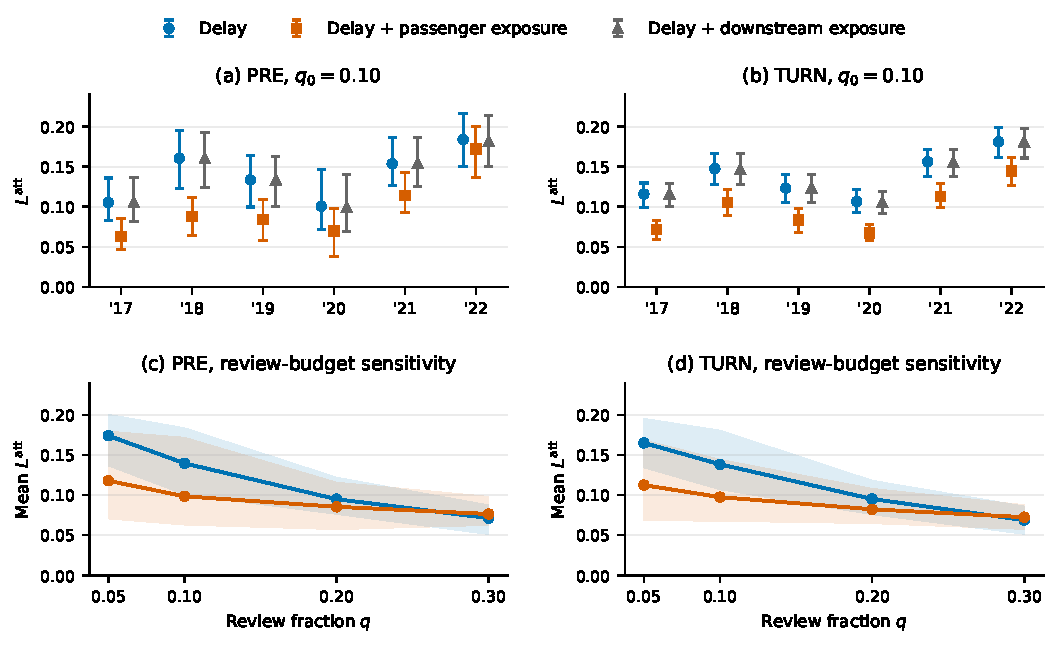
\includegraphics[width=0.99\linewidth]{figures/figure_s5_1_q_boundary.pdf}
\caption{Expected-Delay versus Consequence screening across 2017--2022, separately for PRE (solid) and TURN (hatched). Panel~(a) reports the share of reference shortlist positions displaced by each priority at the nominal review budget $q_0=0.10$; panel~(b) reports the normalized reference-consequence loss $L^{\mathrm{att}}$ at the same budget, with episode-cluster percentile bootstrap intervals ($B=2\,000$) for the Delay priority; panel~(c) reports the review-budget sensitivity of $L^{\mathrm{att}}$ averaged across years, with the full annual range shown as a band.}
\label{fig:q_boundary}
\end{figure}

At the nominal review budget, expected delay displaces 37--53\% of PRE positions and 40--55\% of TURN positions, and the displaced positions carry $L^{\mathrm{att}}=0.101$--$0.184$ of the reference consequence value in PRE and $0.107$--$0.181$ in TURN. The minimum loss occurs in 2020 ($0.1006$, 95\% CI $[0.0712,0.1461]$ in PRE; $0.1068$, $[0.0931,0.1216]$ in TURN) and the maximum in 2022 ($0.1840$, $[0.1506,0.2163]$ in PRE; $0.1811$, $[0.1618,0.1996]$ in TURN). The intervals exclude zero in every year and stage, so the boundary disagreement between the two priorities is not a small-sample artifact: under the nominal 10\% review capacity, 27--76 PRE positions and 154--215 TURN positions change in each year.
% RESULT 5.2-A: audited annual PRE/TURN contrasts and inference intervals are reported above;
% stage-level detail by view is in Supplementary Table~\ref{tab:sup_e1_screening}.

An intermediate Delay+Exposure priority adds admissible historical passenger or downstream exposure references to the expected-delay signal. Adding the passenger exposure reference reduces the screening loss by 6--45\% in PRE and 20--38\% in TURN, leaving $L^{\mathrm{att}}=0.063$--$0.172$ (PRE) and $0.067$--$0.145$ (TURN); a substantial residual boundary disagreement remains in every year, and in 2022 the passenger multiplier removes only a small part of the gap ($0.1840\to0.1721$ in PRE). Adding the downstream propagation reference behaves differently: the resulting priority reproduces the delay shortlist almost exactly, with $|\Delta L^{\mathrm{att}}|\leq0.003$ relative to expected delay in all twelve year-stage settings. The review-budget sensitivity in Fig.~\ref{fig:q_boundary}(c) shows that the disagreement is concentrated at tight review budgets: the year-mean $L^{\mathrm{att}}$ of the delay priority falls from $0.174$ to $0.071$ (PRE) and from $0.165$ to $0.069$ (TURN) as the review fraction increases from $0.05$ to $0.30$, and the Delay+Passenger and Delay priorities converge to within $0.006$ at $q=0.30$ (year-mean gap $0.0051$ in PRE and $0.0037$ in TURN).
% RESULT 5.2-B: matched Delay / Delay+Exposure / Consequence contrasts and q sensitivity
% are reported above. The Delay+Exposure construction (a multiplicative delay-by-exposure
% score using frozen historical references) is fixed before held-out outcome review.
% INTERPRETATION 5.2: expected delay is not substitutable for consequence-based screening
% at the active boundary; passenger exposure recovers part of the difference while the
% downstream exposure reference adds essentially none.

\subsection{Screening Priority and Recoverable Opportunity}
\label{subsec:results_local_recovery}

Consequence-based screening prioritizes baseline disruption exposure, whereas local recovery evaluates the improvement still available after accounting for feasibility and the effort of pursuing an additional effective off-block target. A highly prioritized chain need not have a positive model-optimal recovery target; likewise, recoverable value is not interchangeable with baseline consequence. The relationship is therefore examined using the valid Stage-II population rather than being inferred solely from a consequence-selected shortlist.

For each supported chain-stage case in the annual reference cohort, we obtain the HJ reference target $u^*$, activation indicator $\mathbf 1\{u^*>0\}$, and model-recoverable value $V=J^{HJ}(0)-J^{HJ}(u^*)$. Figure~\ref{fig:stage2_recoverability} reports the resulting activation and recoverable-value distributions under the Balanced objective, together with the objective-wise activation share. Under Balanced, the reference target is positive for 82--92\% of the annual reference cohorts, and the share of cases whose model-recoverable value is exactly zero is 8.4--17.7\%. The median recoverable value per case ranges from 0.018 CU (2017) to 0.136 CU (2018), against annual aggregate reference values $\sum_i V^{HJ}_i$ of 40.4--85.1 CU. Activation is higher in TURN than in PRE in every year (0.83--0.93 versus 0.77--0.88), and the zero-recoverable-value share is correspondingly higher in PRE than in TURN in every year (PRE 0.115--0.229 versus TURN 0.074--0.175).
% RESULT 5.3-A: reference activation and recoverable-value distributions are reported above.
% The association between baseline consequence priority and remaining recoverable value on
% the FULL eligible population C_1, and recovery-opportunity Coverage@K, require Stage-II
% recoverable values outside the annual shortlists and therefore remain pending.

\begin{figure}[pos=t]
\centering
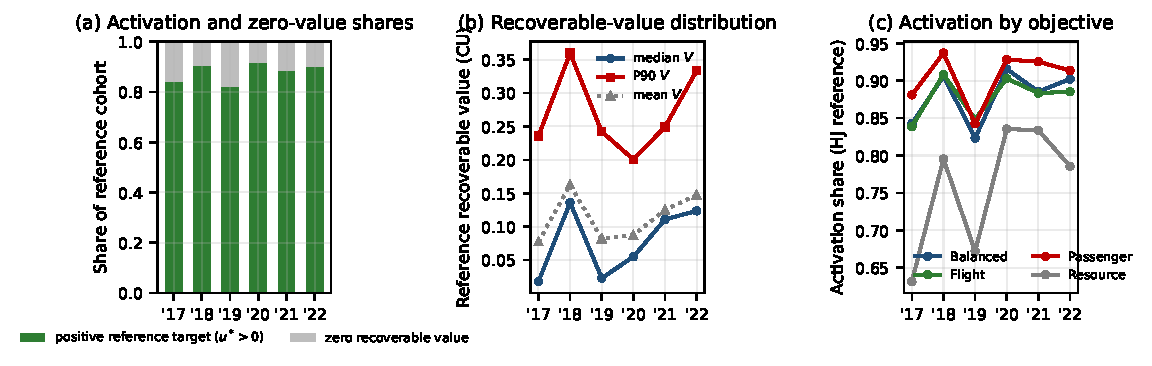
\includegraphics[width=0.99\linewidth]{figures/figure_s5_2_recoverability.pdf}
\caption{Baseline consequence priority and model-recoverable opportunity in the annual Stage-II reference cohorts. Panel~(a) reports the share of cases with a positive History+Joint reference target and the share with zero recoverable value under the Balanced objective; panel~(b) reports median, mean, and P90 per-case recoverable value $V^{HJ}$; panel~(c) reports the activation share under the four prespecified objective-weight settings. All panels use the same annual reference cohorts as Table~\ref{tab:annual_evaluation_support}.}
\label{fig:stage2_recoverability}
\end{figure}

The distributions also document how close the reference decisions are to their decision boundaries: the median gap between the optimal target's objective value and the best alternative is $0.010$--$0.021$ CU across years and objectives, which is the same order as the objective perturbations examined in Section~\ref{subsec:results_objectives}. We therefore do not treat target stability as evidence of information sufficiency anywhere in this section; it is reported alongside the magnitude of the underlying objective gaps.
% RESULT 5.3-B: recovery-opportunity Coverage@K for each screening method is not yet
% computed: it requires reference recoverable values on the full eligible population C_1,
% which the audited outputs provide only for the annual shortlists. The pending quantity
% and its required inputs are named in Supplementary Section~\ref{sup:additional_results}.

\subsection{Decision Effects of Operating Information}
\label{subsec:results_information}

We next examine whether the incremental decision value of operating information differs between the two decision layers. The paired contrasts use History+Joint (HJ) as the reference, with Current+Joint (CJ), History+Point (HP), and History+Marginal (HM) as alternatives. Each comparison fixes the relevant decision epoch, feasible set, objective, and reference evaluator, and is computed on the paired common-support intersection of the two representations at the same stage-specific review capacity. Stage-I shortlist changes and retained consequences are assessed separately from Stage-II recovery activation, target agreement, and reference-objective loss.

Table~\ref{tab:information_decision_summary} reports the annual results for the three principal comparisons. Stage-I $L^{\mathrm{att}}$ and Stage-II $L^{\mathrm{rec}}$ have different reference objects and denominators, so their magnitudes are not treated as a common performance scale.

\begin{table}[pos=t]
\centering
\caption{Six-year decision effects of temporal and probabilistic representations.}
\label{tab:information_decision_summary}
\scriptsize
\setlength{\tabcolsep}{2.6pt}
\begin{tabular}{llrrrr}
\toprule
Year & Contrast & \shortstack{Stage-I displaced\\share of shortlist} & \shortstack{$L^{\mathrm{att}}$ [95\% CI]} & \shortstack{Stage-II exact\\agreement $A_0$} & \shortstack{$L^{\mathrm{rec}}$ [95\% CI]} \\
\midrule
2017 & CJ--HJ & 0.2361 & 0.0320 [0.0255, 0.0392] & 0.342 & 0.6676 [0.6028, 0.7382] \\
 & HP--HJ & 0.8580 & 0.4986 [0.4708, 0.5241] & 0.226 & 0.9145 [0.8780, 0.9447] \\
 & HM--HJ & 0.0192 & 0.0010 [0.0004, 0.0018] & 0.693 & 0.1095 [0.0818, 0.1416] \\
2018 & CJ--HJ & 0.1683 & 0.0233 [0.0180, 0.0292] & 0.239 & 0.6194 [0.5622, 0.6833] \\
 & HP--HJ & 0.8757 & 0.5050 [0.4783, 0.5309] & 0.130 & 0.9814 [0.9718, 0.9892] \\
 & HM--HJ & 0.0191 & 0.0011 [0.0001, 0.0020] & 0.585 & 0.0935 [0.0718, 0.1178] \\
2019 & CJ--HJ & 0.1806 & 0.0253 [0.0214, 0.0330] & 0.353 & 0.6957 [0.6359, 0.7612] \\
 & HP--HJ & 0.8854 & 0.5291 [0.5052, 0.5543] & 0.241 & 0.9321 [0.8975, 0.9616] \\
 & HM--HJ & 0.0194 & 0.0009 [0.0004, 0.0015] & 0.730 & 0.0853 [0.0623, 0.1129] \\
2020 & CJ--HJ & 0.8987 & 0.5060 [0.4820, 0.5285] & 0.086 & 0.9977 [0.9944, 1.0006] \\
 & HP--HJ & 0.8418 & 0.4313 [0.4071, 0.4563] & 0.171 & 0.8963 [0.8721, 0.9192] \\
 & HM--HJ & 0.0127 & 0.0006 [0.0000, 0.0012] & 0.631 & 0.0906 [0.0727, 0.1131] \\
2021 & CJ--HJ & 0.1224 & 0.0101 [0.0075, 0.0134] & 0.495 & 0.3102 [0.2616, 0.3662] \\
 & HP--HJ & 0.8509 & 0.4134 [0.3865, 0.4367] & 0.153 & 0.9535 [0.9365, 0.9680] \\
 & HM--HJ & 0.0249 & 0.0026 [0.0009, 0.0049] & 0.618 & 0.1051 [0.0809, 0.1329] \\
2022 & CJ--HJ & 0.1786 & 0.0244 [0.0180, 0.0299] & 0.299 & 0.5947 [0.5376, 0.6576] \\
 & HP--HJ & 0.8872 & 0.4995 [0.4768, 0.5246] & 0.130 & 0.9575 [0.9388, 0.9741] \\
 & HM--HJ & 0.0376 & 0.0026 [0.0013, 0.0048] & 0.581 & 0.1247 [0.0966, 0.1570] \\
\bottomrule
\end{tabular}
\par\vspace{3pt}
\begin{minipage}{0.98\linewidth}
\footnotesize
Entries use each contrast's paired common-support population at the nominal review budget $q_0=0.10$; all Stage-II quantities use the same annual HJ reference cohort as Table~\ref{tab:annual_evaluation_support}. Interval estimates are episode-cluster percentile bootstrap intervals ($B=2\,000$, seed fixed before the run). Stage-I displaced share is the number of reference shortlist positions replaced, divided by the total shortlist size across PRE and TURN. HM--HJ is interpreted as a dependence-only contrast subject to the weighted-marginal preservation audit reported in the text; $L^{\mathrm{rec}}$ is not intrinsically bounded by one. Absolute reference losses, reference denominators, and activation events are given in the Supplementary Material.
\end{minipage}
\end{table}

The dependence-only contrast is small at both decision layers. Replacing the joint state coupling with the exact weighted-marginal coupling (HM--HJ) displaces 1.3--3.8\% of shortlist positions with $L^{\mathrm{att}}=0.0006$--$0.0026$, and it leaves exact target agreement at $A_0=0.58$--$0.73$ with $L^{\mathrm{rec}}=0.085$--$0.125$. The Stage-I intervals exclude zero in every year, but the retained reference consequence is above 99.6\% throughout. By contrast, collapsing the distribution to the weighted joint medoid (HP--HJ) displaces 84--89\% of shortlist positions with $L^{\mathrm{att}}=0.41$--$0.53$; Stage-II exact agreement falls to $A_0=0.13$--$0.24$ and $L^{\mathrm{rec}}=0.90$--$0.98$. The paired Point-minus-Marginal increment attributes most of this loss to the discarded primitive marginal uncertainty rather than to cross-state alignment: the increment is $L^{\mathrm{att}}=0.41$--$0.53$ and $L^{\mathrm{rec}}=0.80$--$0.89$, and the residual Joint-alignment component is the same small HM--HJ quantity reported above. Restoring marginal uncertainty therefore recovers most of the observed Point-to-Joint difference, while additional joint alignment contributes little at either layer.
% RESULT 5.4-B: paired HP--HJ and validated HM--HJ results are reported above.
% The weighted-marginal audit (Supplementary Section~\ref{sup:states}) verifies exact
% preservation of every weighted primitive marginal for all audited nodes; the coupling
% is a diagnostic product coupling whose physical feasibility is not asserted.

The temporal contrast is year-dependent. Under the Balanced objective the Current representation leaves $L^{\mathrm{att}}$ between $0.010$ (2021) and $0.032$ (2017) in the pre-pandemic years and 2021--2022, but $L^{\mathrm{att}}=0.506$ in 2020 together with $A_0=0.086$ and $L^{\mathrm{rec}}=0.998$: in the disruption year the current-state representation loses almost the entire reference recoverable value on the reference cohort, missing 425 of the 474 activation decisions. The Current and History models are trained with the same architecture size, normalization, protocol, and seed and differ only in the history-encoder mode, so this gap is not attributable to parameter capacity; it is nonetheless an implemented-configuration contrast rather than a pure information-content estimate.
% RESULT 5.4-A: paired CJ--HJ effects are reported above; the matched-capacity control is
% the implemented same-capacity Current comparator described in Section~\ref{subsec:state_reconstruction}.

A component-level audit explains why the dependence-only contrast can be small while the temporal and point contrasts are not. Under the exact marginal coupling, the Flight and Resource domain scores are numerically identical to their Joint counterparts for every audited candidate in all six years (maximum absolute difference below $10^{-13}$ CU), because those components are linear in the unresolved primitives. Only the Passenger domain differs, for 39--66\% of candidates, and it does so through the threshold-event exposures whose probabilities depend on the coupling. Cross-state dependence therefore reaches the two decisions only through threshold-type consequences in this consequence system; this is a property of the specified objective, not a general statement about dependence.
% INTERPRETATION 5.4: the observed pattern is task-specific: dependence changes few
% screening positions and moderate target choices, whereas the temporal representation
% and the discarded marginal uncertainty change both layers substantially.

\subsection{Information Requirements under Alternative Recovery Objectives}
\label{subsec:results_objectives}

The relative value of probabilistic dependence may change with the consequences that the recovery objective emphasizes. To examine this management question, we compare HM and HJ under four prespecified domain-weight settings: Balanced, Flight emphasis, Passenger emphasis, and Resource emphasis. Both targets are recomputed for each objective and evaluated under that objective's own Joint reference. The main comparison fixes the annual reference cohort independently of screening choice and domain weights, so preference changes do not also redefine the analyzed population.

Figure~\ref{fig:objective_dependence} reports the objective-by-distribution comparison. Its primary decision outcomes are exact target agreement, the fraction of cases whose optimal target is dependence-sensitive, and the mean absolute target change; fixed-target objective differences are reported separately.

\begin{figure}[pos=t]
\centering
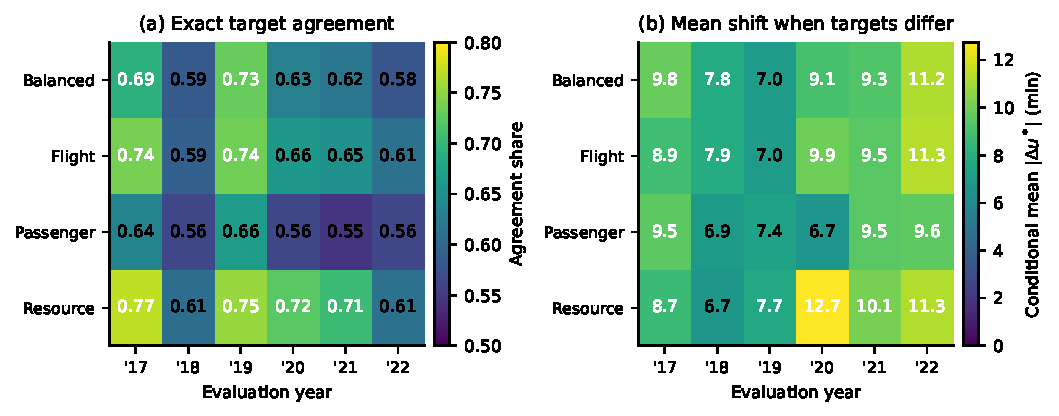
\includegraphics[width=0.99\linewidth]{figures/figure_s5_3_objectives.pdf}
\caption{Decision sensitivity to joint-state dependence under alternative recovery objectives. Panel~(a) reports exact HM--HJ target agreement within each prespecified objective; panel~(b) reports the mean absolute target change $|\Delta u^*|$ across all cases (the median change is zero in every setting); panel~(c) reports the median History+Joint recoverable value under each objective. The same annual reference cohorts are retained throughout.}
\label{fig:objective_dependence}
\end{figure}

Exact target agreement between the marginal and joint decisions ranges from $A_0=0.581$--$0.730$ under Balanced, $0.593$--$0.739$ under Flight emphasis, $0.547$--$0.664$ under Passenger emphasis, and $0.608$--$0.772$ under Resource emphasis. Passenger emphasis is the least stable objective in every year except 2017, and its median recoverable value is the largest of the four settings (0.031--0.256 CU versus 0.004--0.075 CU under Resource emphasis). Resource emphasis changes the composition of the decision problem in the opposite direction: activation is lowest ($0.631$--$0.835$) and the zero-recoverable-value share highest ($0.165$--$0.369$), consistent with the invariance of the Resource component to the local recovery action. No objective produces an invariant ranking across all six years: the largest annual agreement gap between any two objectives is reached in 2018 (Flight $0.739$ versus Passenger $0.564$).
% RESULT 5.5-A: objective-specific paired HM--HJ outcomes and support are reported above;
% year-by-year objective detail is in Supplementary Table~\ref{tab:sup_e3}.

Two mechanism results qualify these differences. First, the mean absolute target change under dependence is 1.8--4.7 minutes, but the median change is zero in all twenty-four year-objective settings, so most agreement is carried by cases where dependence does not move the optimum at all, with a tail of cases moving by 30--45 minutes. Second, the median decision margin is small ($0.010$--$0.021$ CU) relative to the objective perturbations introduced by reweighting domains, so objective-driven changes in target selection should be read together with the margin distribution rather than as evidence that one representation dominates.
% RESULT 5.5-B: the threshold x headroom mechanism ablation is NOT reported here.
% The audited mechanism diagnostic is degenerate on this cohort: every reference-cohort
% case is fully supported by construction (threshold-support change status = UNCHANGED for
% 100% of cases in all six years), and the headroom diagnostic records only the annual
% global parameter. The four prespecified diagnostic structures therefore require a
% dedicated run on a cohort that includes partially supported states, and the threshold
% components' action response remains to be exported.
% INTERPRETATION 5.5: no claim that Passenger emphasis has the greatest dependence value,
% and no claim that Joint is uniformly superior. Resource emphasis changes decision
% composition through the invariant Resource component and the recovery-effort term.

\subsection{Operating-stage and Regime Differences}
\label{subsec:results_heterogeneity}

The preceding analyses use annual evidence throughout rather than treating additional years as an appendix to a 2019 benchmark. This final subsection considers which relationships vary with the operating environment, without repeating the full annual metric tables. We compare PRE with TURN and examine annual contrasts in the pre-pandemic operating years (2017--2019), the pandemic disruption year (2020), and the recovery years (2021--2022). Differences are interpreted with their stage composition, eligibility, and evaluation scales; they do not isolate a causal effect of the pandemic or any particular external shock.

Screening disagreement between expected delay and consequence is lower in the pre-pandemic benchmark and in 2020 than in the recovery years, for both stages: the delay priority's $L^{\mathrm{att}}$ averages $0.133$ (PRE) and $0.129$ (TURN) in 2017--2019, falls to $0.101$ and $0.107$ in 2020, and rises to $0.169$ in both stages across 2021--2022. The same ordering appears in the paired Stage-I displacement: delay replaces 39--46\% of positions in the earlier years and 52--55\% in 2021--2022. Loss magnitudes and population sizes move in opposite directions in 2020: the PRE candidate population contracts to 675 while the PRE screening loss reaches its six-year minimum.
% RESULT 5.6-A: supported annual/stage and regime contrasts based on E1--E3 primary
% estimates are reported above and in Supplementary Tables~\ref{tab:sup_e1_screening}
% and~\ref{tab:sup_support_matrix}.

The representation contrasts vary less by stage than by year. Under the Balanced objective, HM--HJ loses $L^{\mathrm{rec}}=0.085$--$0.093$ in 2017--2019, $0.091$ in 2020, and $0.105$--$0.125$ in 2021--2022, while HP--HJ loses $0.90$--$0.98$ throughout; the ordering of the three contrasts is identical in all six years and both stages. The Current representation is the exception: its Stage-II loss is $0.31$--$0.70$ in the pre-pandemic and recovery years and $0.998$ in 2020, where its missed-activation count (425 of 474 reference-cohort cases) accounts for nearly the entire loss. Objective-level agreement is equally year-specific: HM--HJ target agreement under Balanced falls from $0.730$ (2019) and $0.631$ (2020) to $0.581$ (2022), with Passenger emphasis remaining the least stable setting.
% RESULT 5.6-B: within-chain rolling-epoch trajectories are NOT reported here: the
% audited six-year outputs evaluate prespecified canonical epochs only, and the C_3
% rolling-epoch analysis requires a separate pass over all admissible epochs. Where
% adequate support exists it will be added to Supplementary Section~\ref{sup:additional_results}.
% INTERPRETATION 5.6: operating-stage and annual differences are described within the
% annual evaluation systems; no mechanism is claimed for the 2020 contrasts.

% Existing result-layer summary labels preserved for compatibility:
%   sec:results, subsec:results_screening, subsec:results_local_recovery,
%   subsec:results_information, tab:information_decision_summary,
%   fig:q_boundary, fig:stage2_recoverability.
% Supplemental tables and year-by-year diagnostics: Section~\ref{sup:additional_results}.
